  \section[Cloud]{Le Cloud : vue d'ensemble}

  \subsection[Cloud]{Le Cloud : les concepts}

  \begin{frame}
    \frametitle{Le cloud, c'est large !}
    \begin{itemize}
      \item Stockage/calcul distant \pause (on oublie, cf. externalisation)\pause
      \item Virtualisation++\pause
      \item Abstraction du matériel (voire plus)\pause
      \item Accès normalisé par des APIs\pause
      \item Service et facturation à la demande\pause
      \item Flexibilité, élasticité
    \end{itemize}
  \end{frame}

  \begin{frame}
    \frametitle{WaaS : Whatever as a Service}
    \begin{itemize}
      \item Principalement\pause
      \begin{description}
        \item[IaaS] Infrastructure as a Service\pause
        \item[PaaS] Platform as a Service\pause
        \item[SaaS] Software as a Service\pause
      \end{description}
      \pause
      \item Mais aussi :
      \pause
      \begin{itemize}
        \item Database as a Service
        \item Network as a Service
        \item Load balancing as a Service\pause
        \item \$APPLICATION as a Service
      \end{itemize}
    \end{itemize}
  \end{frame}

  \begin{frame}
    \frametitle{Le cloud en un schéma}
    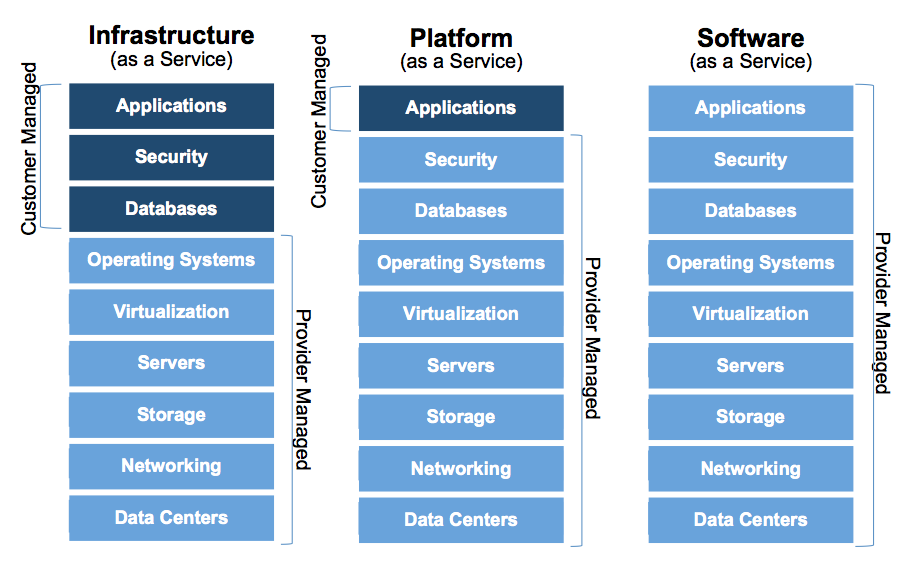
\includegraphics[width=\linewidth,height=\textheight]{images/cloud.png}
  \end{frame}

  \begin{frame}
    \frametitle{Pourquoi du cloud ? Côté technique}
    \begin{itemize}
      \item Abstraction des couches plus basses
      \item On peut tout programmer à son gré
      \item Permet la mise en place d'architectures scalables
    \end{itemize}
  \end{frame}

  \begin{frame}
    \frametitle{Virtualisation dans le cloud}
    \begin{itemize}
      \item Le cloud IaaS repose souvent sur la virtualisation
      \item Ressources compute $\leftarrow$ virtualisation
      \item Virtualisation complète : KVM, Xen
      \item Virtualisation conteneurs : OpenVZ, LXC, Docker
    \end{itemize}
  \end{frame}

  \begin{frame}
    \frametitle{Notions et vocabulaire IaaS}
    \begin{itemize}
      \item L'instance est par définition éphémère
      \item Elle doit être utilisée comme ressource de calcul
      \item Séparer les données des instances
    \end{itemize}
  \end{frame}

  \subsection[Orchestration]{Orchestrer ses ressources}

  \begin{frame}
    \frametitle{Pourquoi orchestrer ?}
    \begin{itemize}
      \item Définir tout une infrastructure dans un seul fichier texte
      \item Autoscaling
        \item Adapter ses ressources en fonction de ses besoins en temps réel
    \end{itemize}
  \end{frame}

  \subsection[Conteneurs]Aller encore plus loin}

  \begin{frame}
    \frametitle{Encore plus "cloud" qu'une instance}
    \begin{itemize}
      \item Partage du kernel
      \item Un seul process par conteneur
    \end{itemize}
  \end{frame}

  \begin{frame}
    \frametitle{Le kernel Linux}
    \begin{itemize}
      \item Namespaces
      \item cgroups
    \end{itemize}
  \end{frame}

 \begin{frame}
     \frametitle{Les namespaces}
    \begin{itemize}
      \item Mount
      \item Network
      \item PID
      \item Hostname
      \item User
    \end{itemize}
  \end{frame}

\begin{frame}
     \frametitle{Systèmes de conteneurs}
    \begin{itemize}
      \item Docker
      \item LXC
      \item Rocket
    \end{itemize}
  \end{frame}
